\documentclass[17pt]{beamer} %Makes presentation
%\documentclass[handout]{beamer} %Makes Handouts
\usetheme{Singapore} %Gray with fade at top
\useoutertheme[subsection=false]{miniframes} %Supppress subsection in header
\useinnertheme{rectangles} %Itemize/Enumerate boxes
\usecolortheme{seagull} %Color theme
\usecolortheme{rose} %Inner color theme

\definecolor{light-gray}{gray}{0.75}
\definecolor{dark-gray}{gray}{0.55}
\setbeamercolor{item}{fg=light-gray}
\setbeamercolor{enumerate item}{fg=dark-gray}

\setbeamertemplate{navigation symbols}{}
%\setbeamertemplate{mini frames}[default]
%\setbeamercovered{dynamics}
\setbeamerfont*{title}{size=\Large,series=\bfseries}
\setbeamerfont{footnote}{size=\tiny}

%\setbeameroption{notes on second screen} %Dual-Screen Notes
%\setbeameroption{show only notes} %Notes Output

\setbeamertemplate{frametitle}{\vspace{.5em}\bfseries\insertframetitle}
\newcommand{\heading}[1]{\noindent \textbf{#1}\\ \vspace{1em}}

\usepackage{bbding,color,multirow,times,ccaption,tabularx,graphicx,verbatim,booktabs}
\usepackage{colortbl} %Table overlays
\usepackage[english]{babel}
%\usepackage[latin1]{inputenc}
%\usepackage[T1]{fontenc}
\usepackage{lmodern}

%\author[]{Thomas J. Leeper}
\institute[]{
  \inst{}%
  Department of Government\\London School of Economics and Political Science
}

\usepackage{tikz}
\usetikzlibrary{shapes,arrows,decorations.pathreplacing,calc}

\title{Ethics and Research Integrity}

\date[]{}

\begin{document}

\frame{\titlepage}

\frame{\tableofcontents}

\section{Review ITS}
\frame{\tableofcontents[currentsection]}

% Interrupted time-series

\frame<1>[label=itshow]{
	\frametitle{How ITS Works}
	\begin{itemize}\itemsep0.5em
		\item Identify an exogenous shock in $X$ that might affect $Y$
		\item Look at $Y$ before ($t$) and after ($t+1$) the shock
		\item We only observe one manifest outcome at each point in time
		\item<2-> To make a causal inference, we need:
			\begin{itemize}
				\item $Y_{0,t}$ and $Y_{1,t}$, or
				\item $Y_{0,t+1}$ and $Y_{1,t+1}$
			\end{itemize}
		\item<2-> Use pre-post comparisons to infer the value of unobserved potential outcomes		
	\end{itemize}
}

\frame<1-2>[label=its]{
	\begin{center}
	\begin{tikzpicture}[scale=0.7]
    \draw[->] (0,0) -- (11,0) node[right] (xaxis) {\small time};
    \draw[->] (0,0) -- (0,11) node[left] (yaxis) {};
    % x ticks
    \foreach \x in {1,2,...,10}
       	\draw (\x,1pt) -- (\x,-3pt) node[anchor=north] {};
    % y ticks
    \foreach \y in {0,...,10}
         \draw (1pt,\y) -- (-3pt,\y) node[anchor=east] {};
    % intervention
    \draw (5.5,-0.25) node[below, scale=0.5] (IV) {Intervention};
    \draw (5.5,0) -- (5.5,11);

	\draw<1>[thick,blue] (5,10) -- (6,7);
	\draw<2->[dashed,thick,blue] (5,10) -- (6,7);
	\draw<2->[thick,blue] (1,4) -- (2,2) -- (3,5) -- (4,3) -- (5,10);
	\draw<2->[thick,blue] (6,7) -- (7,6) -- (8,6) -- (9,4) -- (10,3);
	
	\draw<3->[thick,red] (1,8) -- (2,8.5) -- (3,7.5) -- (4,8.5) -- (5,8) -- (6,7.5) -- (7,8.5) -- (8,8) -- (9,8.5) -- (10,7.5);
	\end{tikzpicture}
	\end{center}
}

\againframe<1-2>{itshow}


\frame{
	\begin{center}
	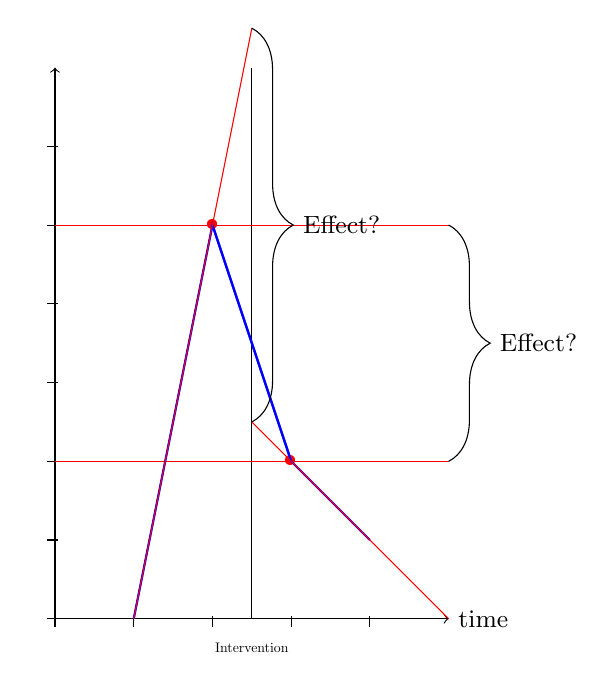
\begin{tikzpicture}[scale=1]
    \draw[->] (0,0) -- (5,0) node[right] (xaxis) {\small time};
    \draw[->] (0,0) -- (0,7) node[left] (yaxis) {};
    % x ticks
    \foreach \x in {0,...,4}
       	\draw (\x,1pt) -- (\x,-3pt) node[anchor=north] {};
    % y ticks
    \foreach \y in {0,...,6}
         \draw (1pt,\y) -- (-3pt,\y) node[anchor=east] {};
    % intervention
    \draw (2.5,-0.25) node[below, scale=0.5] (IV) {Intervention};
    \draw (2.5,0) -- (2.5,7);

	\draw[thick,blue] (2,5) -- (3,2);
	\node<2-> [red] at (2,5) {\small \textbullet};
	\node<2-> [red] at (3,2) {\small \textbullet};
	
	\draw<3-5>[red] (0,5) -- (5,5);
	\draw<3-5>[red] (0,2) -- (5,2);
	\draw<4-5>[right,decorate,decoration={brace, amplitude=15pt}] (5,5) -- (5,2) node[right, xshift=15pt, pos=0.5] (diff) {\small Effect?};
	        
	\draw<5->[thick,blue] (1,0) -- (2,5) -- (3,2) -- (4,1);
	\draw<6->[red] (1,0) -- (2.5,7.5);
	\draw<6->[red] (2.5,2.5) -- (5,0);
	\draw<7->[right,decorate,decoration={brace, amplitude=15pt}] (2.5,7.5) -- (2.5,2.5) node[right, xshift=15pt, pos=0.5] (diff) {\small Effect?};
	
	\end{tikzpicture}
	\end{center}
}

\frame{
	\frametitle{Difference-In-Differences}
	\small
	\begin{itemize}\itemsep0.5em
		\item How do we know change in $Y$ wasn't due to something else?
			\begin{itemize}
				\item How do we know $Y_{0,t}$ is a good stand-in for $Y_{0,t+1}$?
			\end{itemize}
		\item<2-> Use a comparison case (or cases)!
		\item<3-> Instead of using the pre-post difference in $Y_i$ to estimate the causal effect, use the difference in pre-post differences for two units $i$ and $j$:
		\begin{align*}
		(Y_{i,t+1} - Y_{i,t}) - (Y_{j,t+1} - Y_{j,t})
		\end{align*}
	\end{itemize}
}


\frame{
	\begin{center}
	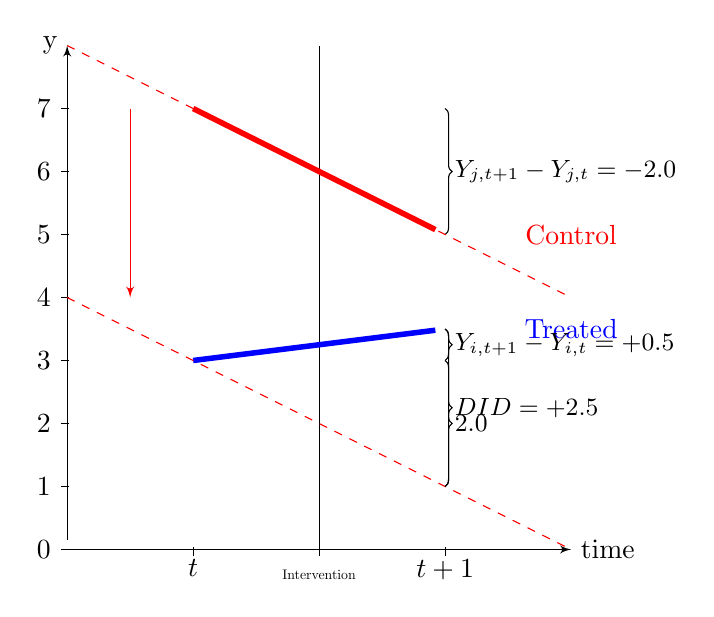
\begin{tikzpicture}[>=latex', scale=0.8]
        \draw[->] (0,0) node (origin) {}  -- (8,0) node[right] (xaxis) {time};
        \draw[->] (origin) -- (0,8) node[left] (yaxis) {y};
        % x ticks
        \foreach \x in {2,4,6}
        	\draw (\x,1pt) -- (\x,-3pt) node[anchor=north] {};
        \draw (2,0) node[below] (before) {$t$};
        \draw (6,0) node[below] (after) {$t+1$};
        \draw (4,-0.25) node[below, scale=0.5] (IV) {Intervention};
        % y ticks
        \foreach \y in {0,...,7}
             \draw (1pt,\y) -- (-3pt,\y) node[anchor=east] {$\y$};
        % intervention
        \draw (4,0) -- (4,8);

        % line
        \draw<2-> (6,3.5) node (tr) {};
        \draw<3-> (6,5) node (ctrl) {};
        \draw<2-3>[blue] (8,3.5) node (trlab) {Treated};
        \draw<3-3>[red] (8,5) node (ctrllab) {Control};        
        \draw<2->[blue, line width=2pt] (2,3) -- (tr);
        \draw<3->[red, line width=2pt] (2,7) -- (ctrl);
        
        % diffs
        \draw<4-6>[right,decorate,decoration={brace,mirror}] 
        	(6,3) -- (6,3.5) node[right, pos=0.5] (idiff) {\small $Y_{i,t+1} - Y_{i,t} = +0.5$};
        \draw<4-6>[right,decorate,decoration={brace}] 
            (6,7) -- (6,5) node[right, pos=0.5] (jdiff) {\small $Y_{j,t+1} - Y_{j,t} = -2.0$};
        
        % trends
        \draw<5-6>[red,->] (1,7) -- (1,4);
        \draw<5->[red, dashed] (0,8) -- (8,4);
        \draw<5->[red, dashed] (0,4) -- (8,0);
        \draw<6>[right,decorate,decoration={brace}] 
            (6,3) -- (6,1) node[right, pos=0.5] (idiff2) {\small $2.0$};
        \draw<7>[right,decorate,decoration={brace}] 
            (6,3.5) -- (6,1) node[right, pos=0.5] (idiff2) {\small $DID = +2.5$};
                        
        
    \end{tikzpicture}
    \end{center}
}

\frame{

	\frametitle{Threats to Validity}
	\begin{enumerate}
	\item History
	\item Maturation
	\item Testing
	\item Instrumentation
	\item Instability
	\item Regression to the mean
	\end{enumerate}
}
% history: stimultaneous alterntive cause
% maturation: time trends
% testing: measurement changes behavior
% instrumentation: operationalization changes over time
% instability: measurement error
% regression (to the mean):
% - statistically: extreme cases will be less extreme on second measurement
% - in policy terms: interventions are most likely when problems are extreme

% one more not mentioned by Campbell and Ross: If the series is an aggregation, it's also possibly due to attrition or changing composition of the sample from which the data is aggregated


\frame{}


\section{Ethics}
\frame{\tableofcontents[currentsection]}

\frame{
\frametitle{History: Key Moments}

\small

\begin{enumerate}
\item Tuskegee (1932-1972) and Guatemala (1946-1948) Studies
\item Nuremberg Code (1947)
\item Helsinki Declaration (1964)
\item U.S. 45 CFR 46 (1974) and ``Common Rule'' (1991)
\item The Belmont Report (1979)
\item EU Data Protection Directive (1995; 2012)
	\begin{itemize}
	\item UK Data Protection Act (1998)
	\end{itemize}
\end{enumerate}
}


\frame{
	\frametitle{Helsinki Declaration}
	
	\small
	\begin{itemize}
	\item Adopted by the World Medical Association in 1964\footnote{\url{http://www.bmj.com/content/2/5402/177}}
	\item Narrowly focused on medical research
	\item Expanded the Nuremberg Code
		\begin{itemize}
		\item Relaxed consent requirements
		\item Risks should not exceed benefits
		\item Institutionalization of ethics oversight
		\end{itemize}
	\item<2-> Do these rules apply to non-experimental research? To non-medical research?
	\end{itemize}

}

\frame{
	\frametitle{Social Science Examples}
	\begin{enumerate}\itemsep2em
	\item \href{https://www.youtube.com/watch?v=yr5cjyokVUs}{Milgram Obedience Study (1961)}
	\item \href{https://www.youtube.com/watch?v=760lwYmpXbc}{Stanford Prison Study (1971)}
	\end{enumerate}
}


\frame{
	\frametitle{The Belmont Report}
	
	\small
	\begin{itemize}
	\item Commissioned by the U.S. Government in 1979\footnote{\url{http://www.hhs.gov/ohrp/humansubjects/guidance/belmont.html}}
	\item Three overarching principles:
		\begin{enumerate}
		\item Respect for persons
		\item Beneficence
		\item Justice
		\end{enumerate}
	\item Three policy implications:
		\begin{itemize}
		\item Informed consent
		\item Assessment of risks/benefits
		\item Care for vulnerable populations
		\end{itemize}
	\end{itemize}

}


\frame{
	\frametitle{Informed Consent}
	\begin{itemize}
	\item Persons must consent to being a research subject
	\item<2-> What this means in practice is complicated
		\begin{itemize}
		\item What is research?
		\item What is consent?
		\item What is ``informed'' consent?
		\end{itemize}
	\item<3-> Cross-national variations
		\begin{itemize}
		\item Consent forms required in U.S.
		\item Not required in UK
		\end{itemize}
	\end{itemize}

}

\frame{
\frametitle{Benefits and Harm}
	\begin{itemize}\itemsep2em
	\item What is a ``benefit''?
	\item What is a ``harm''?
	\item How do we balance the two?
	\end{itemize}
}


\frame{
	\frametitle{Privacy}
	\begin{itemize}
	\item EU Data Protection Directive (1995) and UK Data Protection Act (1998)
	\item Deals with ``personal data''
	\item Data can be processed when:
		\begin{itemize}
		\item Consent is given
		\item Data are used for a ``legitimate'' purpose
		\item Anonymous or confidential
		\end{itemize}
	\item Data cannot leave the EU except under conditions
	\end{itemize}
}


\frame{
	\frametitle{{\normalsize Lots of Other Ethical Questions}}
	\begin{enumerate}
	\item<2-> Funding
	\item<3-> Independence and Politicization
	\item<4-> Vulnerable populations (e.g. children, sick)
	\item<5-> Cross-national research
	\item<6-> Participant-observation disclosures
	\item<7-> End uses/users of research
	\item<8-> Others?
	\end{enumerate}
}




\frame{
\frametitle{Research Ethics at LSE}

\begin{itemize}
\item Ethics Code \footnote{\url{http://www.lse.ac.uk/intranet/LSEServices/ethics/home.aspx}}
\item Research Ethics Policy \footnote{\url{http://www.lse.ac.uk/intranet/LSEServices/policies/pdfs/school/resEthPolPro.pdf}}
\item Levels of review:
	\begin{enumerate}
	\item Staff: Self-certification
	\item Students: Supervisor certification
	\item LSE Research Ethics Committee
	\item External review
	\end{enumerate}
\end{itemize}

}


\frame{

\begin{center}
\href{http://www.lse.ac.uk/intranet/researchAndDevelopment/researchDivision/policyAndEthics/ethics-annexC.pdf}{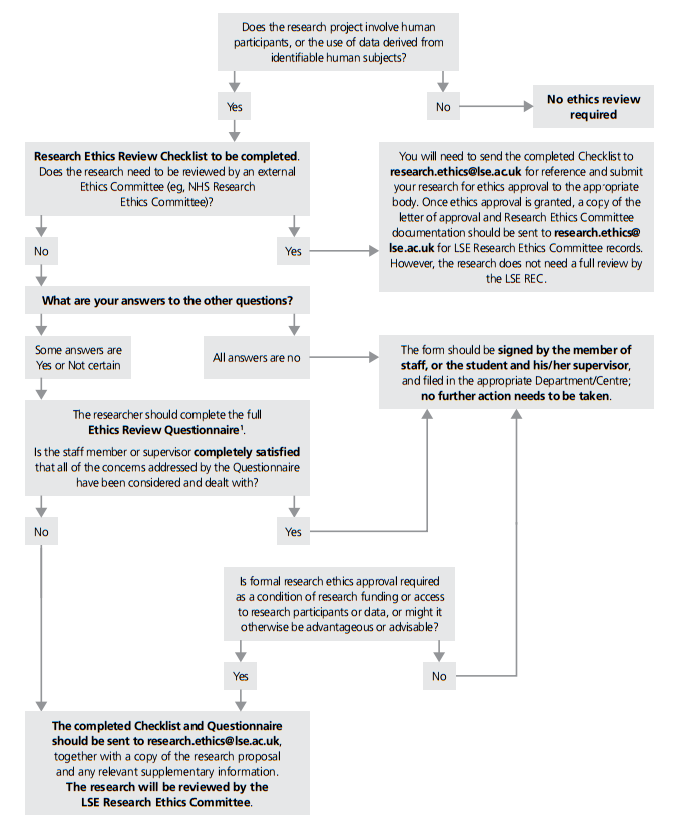
\includegraphics[width=\textwidth]{images/lse_ethics_flowchart}}
\end{center}

}

\frame{
\frametitle{Ethics at LSE}

\begin{itemize}
\item Complete an LSE Ethics form for your proposed research project
\end{itemize}

}


\frame{}


\section{Course Feedback and Redesign}
\frame{\tableofcontents[currentsection]}

\frame{
	
	\begin{itemize}\itemsep1em
	\item What did you like about this course?
	\item What would you change?
	\end{itemize}
	
}

\appendix
\frame{}

\end{document}
